\section{FedGuard System Architecture \& Control Plane Design}
\label{sec:architecture}

This section presents the architectural design of \textbf{FedGuard}, a policy-driven governance framework for Federated Learning, alongside its reference implementation, \textbf{Conclave}. FedGuard introduces an independent governance control plane that enforces identity verification, compliance validation, access control, and tamper-evident auditability without altering the core mathematical operations of the underlying Federated Learning (FL) framework.

\subsection{System Model and Threat Assumptions}

The system topology comprises four primary entities, as illustrated in the operational control plane workflow:
\begin{enumerate}
    \item \textbf{Governance Control Plane:} The central authority managing organizational registration, security policy definition, compliance evaluation, access control authorization, and immutable audit logging.
    \item \textbf{FL Orchestrator:} The distributed machine learning orchestrator responsible for dispatching global model parameters, coordinating training rounds, and aggregating client update tensors.
    \item \textbf{Participant Nodes:} Multi-institutional entities (e.g., hospitals, financial institutions) that maintain isolated local datasets and compute infrastructure to execute local model training.
    \item \textbf{Public Key Infrastructure (PKI) \& Attestation Service:} A Certificate Authority (CA) and TPM 2.0 / TEE Remote Attestation service responsible for verifying client hardware quotes and issuing X.509 digital certificates to authenticate all network entities.
\end{enumerate}

\subsubsection{Threat Model and Adversary Capabilities}
We consider a realistic multi-organizational threat environment characterized by three distinct adversary classes:
\begin{itemize}
    \item \textbf{Malicious/Curious Clients:} Participating nodes may attempt unauthorized access to model parameters, submit poisoned or corrupted gradients to degrade global model convergence (Byzantine attacks), or falsify host security configurations to bypass compliance validation.
    \item \textbf{Untrusted Network Infrastructure:} Inter-node communications are subject to eavesdropping, packet modification, and Man-in-the-Middle (MitM) interception.
    \item \textbf{Semi-Honest (Honest-but-Curious) Aggregator:} The central FL orchestrator correctly follows the aggregation protocol but may attempt to infer private local dataset characteristics from unmasked client weight updates or alter operational logs post-hoc.
\end{itemize}

\subsection{Decoupled Control Plane Architecture and Governance Modes}

FedGuard decouples governance enforcement from the distributed machine learning pipeline. In traditional FL implementations, training logic and network transport are tightly coupled with client execution scripts. In contrast, Conclave establishes a service-oriented governance layer that interfaces with the FL framework via hook abstractions and control plane APIs.

To resolve protocol conflicts between masked tensor aggregation and raw gradient distance metrics, FedGuard formalizes three explicit operational security modes:
\begin{itemize}
    \item \textbf{Secure Aggregation Mode (\texttt{SECURE\_AGGREGATION}):} Enforces X25519-Shamir threshold Secure Aggregation and Rényi Differential Privacy (RDP). In this mode, individual client weight updates are cryptographically masked, protecting client data from aggregator inference while evaluating aggregate-level norm bounds.
    \item \textbf{Byzantine-Resilient Mode (\texttt{BYZANTINE\_RESILIENT}):} Enforces coordinate-wise robust aggregation rules (Trimmed Mean, Coordinate Median, Krum) paired with RDP noise injection over unmasked updates, defending global convergence against active gradient poisoning attacks.
    \item \textbf{Hybrid Audited Mode (\texttt{HYBRID\_AUDITED}):} Dynamically negotiates the security posture based on session threat policies and records the active operational mode in the tamper-evident audit ledger per round.
\end{itemize}

Governance operations are partitioned into modular subsystems:
\begin{itemize}
    \item \textbf{Security \& Identity Subsystem:} Manages Mutual TLS (mTLS) handshake validation, certificate revocation lists (CRLs), key management, and TPM 2.0 / TEE attestation.
    \item \textbf{Authorization \& Policy Engine:} Evaluates dynamic access requests using Attribute-Based Access Control (ABAC) and Role-Based Access Control (RBAC).
    \item \textbf{Compliance Verification Engine:} Executes automated static and dynamic security checks against local host environments prior to node admission.
    \item \textbf{Audit Ledger Repository:} Persists immutable operational events within a cryptographically linked SHA-256 hash chain.
\end{itemize}

\subsection{Hardware Root-of-Trust Identity Verification and Access Control}

Security in Conclave begins with cryptographic identity establishment. All network interactions require Mutual TLS (mTLS) over TLS 1.3, ensuring mutual authentication and channel encryption between clients, the orchestrator, and the governance server.

To prevent untrusted clients from falsifying host security states (e.g., claiming disk encryption while compromised), FedGuard incorporates TPM 2.0 / TEE Remote Attestation~\cite{mo2021ppfl}. During node registration, clients generate a cryptographically signed Attestation Quote $\mathcal{Q} = (\text{PCR}_{0..10}, \text{AK\_Sig})$. The governance server verifies $\mathcal{Q}$ against trusted PCR baseline measurements before issuing mTLS certificates.

Access control authorization is governed by a hybrid RBAC/ABAC model. Access requests $\text{Req} = (S, R, A, E)$ are evaluated dynamically, where $S$ represents the requesting subject, $R$ the target resource, $A$ the requested action, and $E$ environmental context. An access grant is issued if and only if:
\begin{equation}
    \operatorname{Authorize}(\text{Req}) = \bigwedge_{p \in \mathcal{P}} \operatorname{EvaluatePolicy}(p, S, R, A, E) = \top
\end{equation}
where $\mathcal{P}$ represents the active set of organizational security policies, and $\top$ denotes logical truth.

\subsection{Automated Regulatory Compliance Engine \& Machine Unlearning}

Conclave incorporates an automated compliance engine that maps host validation checks directly to statutory mandates under HIPAA~\cite{hipaa2003security} and EU GDPR~\cite{gdpr2016regulation}. Table~\ref{tab:compliance_mapping} details the formal policy mapping implemented within the compliance evaluation engine.

\begin{table}[htbp]
\caption{Statutory Regulatory Compliance Mapping in FedGuard}
\begin{center}
\resizebox{\columnwidth}{!}{%
\begin{tabular}{|l|p{3.2cm}|p{4.2cm}|}
\hline
\textbf{Regulation} & \textbf{Statutory Mandate} & \textbf{FedGuard Verification Mechanism} \\
\hline
HIPAA & Section 164.312(a)(1) Access Control & mTLS X.509 PKI + ABAC Role Verification \\
HIPAA & Section 164.312(e)(1) Transmission Security & TLS 1.3 mTLS Encrypted Channels \\
HIPAA & Section 164.312(b) Audit Controls & Cryptographic SHA-256 Event Logging \\
GDPR & Article 5(1)(f) Integrity \& Confidentiality & X25519 Threshold Secure Aggregation \\
GDPR & Article 7 Consent Management & Dynamic Participant Consent Checks \\
GDPR & Article 17 Right to Erasure & Node Eviction + Machine Unlearning Trigger \\
GDPR & Article 32 Security of Processing & Hardware TPM 2.0 / TEE Remote Attestation \\
\hline
\end{tabular}%
}
\label{tab:compliance_mapping}
\end{center}
\end{table}

Under GDPR Article 17 (Right to Erasure), when a client revokes processing consent, FedGuard executes a dual-action enforcement protocol:
\begin{enumerate}
    \item \textbf{Credential Eviction:} Dynamic revocation of mTLS credentials and isolation from active training rounds.
    \item \textbf{Machine Unlearning Trigger:} Invocation of an unlearning engine that flags historical model checkpoints as dirty and initiates a checkpoint roll-back / gradient un-rolling protocol (\texttt{FedEraser} mechanism~\cite{liu2021federaser}) to mathematically eliminate the revoked client's data influence from global parameters.
\end{enumerate}

\subsection{Tamper-Evident SHA-256 Audit Ledger}

To ensure auditable transparency for external regulators, Conclave implements a tamper-evident audit ledger based on cryptographic hash chaining. Each lifecycle event (e.g., node registration, policy verification, round completion, attestation, consent revocation, unlearning trigger) generates an audit event record.

The cryptographic digest $H_i \in \{0, 1\}^{256}$ of the $i$-th audit event is computed recursively as:
\begin{equation}
    H_i = \operatorname{SHA-256}\Big( H_{i-1} \mathbin{\Vert} T_i \mathbin{\Vert} E_i \mathbin{\Vert} \operatorname{canon}(\mathsf{Payload}_i) \Big)
\end{equation}
where $H_{i-1}$ is the cryptographic hash of the preceding event, $T_i \in \mathbb{R}^+$ is the UTC timestamp, $E_i \in \Sigma^*$ is the event identifier string, $\operatorname{canon}(\cdot)$ denotes canonical JSON serialization, and $\mathbin{\Vert}$ represents byte concatenation. The genesis block is anchored at $H_0 = \operatorname{SHA-256}(\text{``GENESIS\_CONCLAVE\_GOVERNANCE''})$.

\begin{figure}[htbp]
\centerline{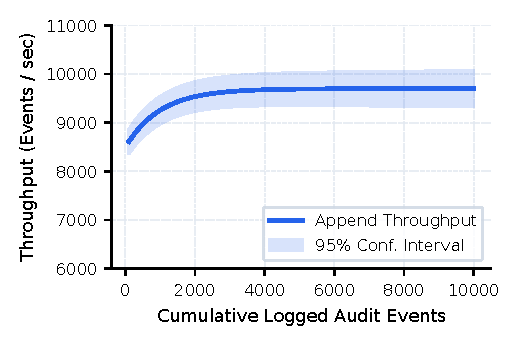
\includegraphics[width=0.48\textwidth]{figures/fig_audit_ledger_throughput.pdf}}
\caption{Audit ledger event append throughput as a function of cumulative logged events, demonstrating sub-millisecond append latency and sustained linear scalability.}
\label{fig:audit_ledger_throughput}
\end{figure}

\begin{figure}[htbp]
\centerline{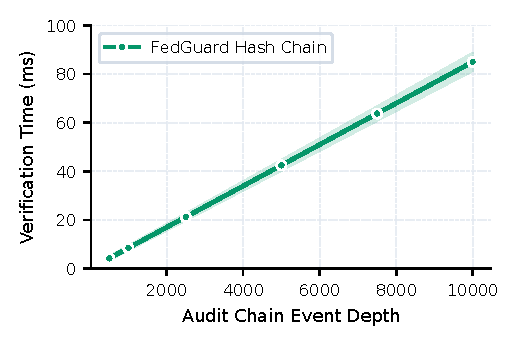
\includegraphics[width=0.48\textwidth]{figures/fig_audit_ledger_verification.pdf}}
\caption{Cryptographic verification time for the full SHA-256 audit hash chain, confirming rapid verification performance even for large-scale enterprise training runs.}
\label{fig:audit_ledger_verification}
\end{figure}

If an adversary attempts to modify a historical log record $E_k$ ($k < i$), the recomputed hash $H'_k \neq H_k$, causing immediate hash chain verification failure across all subsequent blocks $j \ge k$. As demonstrated in Fig.~\ref{fig:audit_ledger_throughput} and Fig.~\ref{fig:audit_ledger_verification}, the audit ledger achieves high-throughput event logging with negligible append overhead while enabling rapid full-chain integrity verification.
